\documentclass[logo,magister, dosguias]{tesis-postgrado}
% opciones: logo,dosguias,magister,doctorado,propuesta,txfonts

\keywords{SPS;Elasticidad;Algoritmo reactivo;Algoritmo predictivo}

\begin{document}
\baselineskip 23pt

% ----------------------------------------------------------
% ----------- PARTE INICIAL --------------------------------
\thispagestyle{empty}
\facultad{Ingeniería}
\departamento{Ingeniería Informática}
\grado{Magíster en Ingeniería Informática}

\titulo{Modelo elástico de replicación de operadores para un sistema de procesamiento de \textit{stream} en tiempo real}

\autor{Daniel Pedro Pablo Wladdimiro Cottet}
\email{daniel.wladdimiro@usach.cl}
\annoingreso{2014}

\fecha{Lunes}{21}{Septiembre}{2015}

\profesorguia{Nicolás Andrés Hidalgo Castillo}
\profesorcoguia{Erika Susana Rosa Olivos}

\ciudad{Santiago}
\pais{Chile}

\makecubierta
\makecopyright

% ----------------------------------------------------------
% ----------- PRIMERA PARTE --------------------------------
\frontmatter
% ### Resumen e Indices ####

\dedicatoria{
Gracias a la vida que me ha dado tanto\\
Me ha dado la risa y me ha dado el llanto,\\
Así yo distingo dicha de quebranto\\
Los dos materiales que forman mi canto\\
Y el canto de ustedes que es el mismo canto\\
Y el canto de todos que es mi propio canto.
}

\begin{agradecimiento}
\small{Me cuesta encontrar las palabras para expresar lo que siento, se cierra un ciclo en mi vida, y con ello una larga traves\'ia de mucho esfuerzo y trabajo, donde espero que de inicio a muchos m\'as. Recib\'i apoyo, cari\~no y paciencia de diferentes personas, las cuales sub\'ian y bajaban de este exc\'entrico tren en cada parada que hac\'iamos, y aunque a veces entre paradas se hac\'ia un viaje muy corto, hab\'ian otras veces que se hac\'ian unos viajes eternos, y no terminaba de distinguir realmente bien d\'onde iba, pero eso daba igual, porque siempre en cada trayecto aprend\'ia y recib\'ia algo de alguna persona, y eso me hizo ir creciendo con el tiempo, lo cual estoy eternamente agradecido. De antemano pido disculpas si me he olvidado de alguien, no fue mi intenci\'on, y espero que pueda agradecerlo en un tiempo futuro. 

Aunque uno a veces siente que todo cambia; la gente, el barrio, la universidad, la sociedad, el trabajo, hay sentimientos y pasiones que nunca cambian, y son esas que te hacen vibrar y llenarte el coraz\'on por estar ah\'i. Sin duda alguna, Izquierda Libertaria es una mis grandes pasiones, donde a trav\'es del FeL me brind\'o una escuela de lucha para poder construir un pueblo digno y soberano. No saben como agradezco estar ah\'i y conocer a mis amigas y amigos que adem\'as son compa\~neras y compa\~neros de lucha: Thomi, Neto, Cachorro, Sussan, Andr\'es, Zarri, Cata, Pato, Cristi\'an, Tuto, Nati, Joaco, Fofi, de coraz\'on gracias por todo su apoyo incondicional. Y m\'as todav\'ia agradezco al FeL porque aqu\'i conoc\'i a mi amada polola, quien no s\'olo le agradezco su apoyo, sino tambi\'en por su cari\~no, alegr\'ia y paciencia, y sin duda todo ser\'ia muy distinto sin ti, no sabes lo agradecido y feliz que soy de estar con vos. Te amo Cami.

Cuando uno va viajando, vas creciendo, vas madurando, te vas dando cuenta que puedes ir resolviendo problemas que antes se hac\'ian imposibles, van d\'andose nuevas herramientas, nuevas habilidades. Por lo mismo es que estoy completamente agradecido de la oportunidad que me brindaron mis queridos profesores gu\'ias Erika y Nicol\'as, porque confiaron en m\'i y se la jugaron por sacar este trabajo, y no s\'olo eso, de abrirme puertas para poder sustentarme y tener un porvenir m\'as tranquilo. De verdad no saben lo orgulloso que estoy de tenerlos como profesores, no s\'olo me han ayudado a formarme como profesional, sino tambi\'en como persona y eso se los agradezco desde el fondo de mi coraz\'on. Tambi\'en agradezco a Pamela, por su apoyo y entrega incondiconal, y la profesora Carolina y el profesor Mauricio, que gracias a CITIAPS me sent\'i en mi segundo hogar, y siento que mucha de las cosas que aprend\'i hoy en d\'ia es gracias a esa peque\~na salita de gran coraz\'on. Y por lo mismo, no puedo olvidar a mi compa\~nero de trabajo, Pablo, siempre me acuerdo como nos conocimos en ese primer d\'ia de las clases de Mag\'ister, nunca cre\'i que gracias a ese saludo pudi\'eramos tener este viaje, donde sali\'o un paper, un proyecto y una bonita amistad, de verdad gracias Pablo, sos un hermano para m\'i. Gracias a todos los que pasaron y est\'an en CITIAPS, \'Alvaro, Jeff, Diego, Farisori, no me olvidar\'e de ustedes, porque sin duda me dejaron marcado y me ayudaron a formarme como profesional y persona. Tambi\'en a mis amigas y amigos de la Usach, Miguel, Gabo, Clau, Karla, Jorge, los quiero caleta y gracias por todo, porque fueron un pilar en mi vida universitaria, donde no los olvidar\'e, porque todo lo que viv\'i con ustedes fue una de mis grandes alegr\'ias.

Pero a veces uno se queda dormido, recuerdas el pasado, y te acuerda que eso fue lo que te form\'o y lo que explica el c\'omo eres hoy en d\'ia. Nunca los voy a olvidar, para mi son mi fuerza, mis ganas, mi apa\~ne, quiz\'a todos estamos en nuestras vidas, pero los tengo mas presente que nunca, Jos\'e, Eduardo, Rub\'en y Felipe, los quiero demasiado. Y como te voy a olvidar, si sos mi hermano de leche, Sim\'on, no s\'olo te tengo que agradecer, te deber\'ia hacer una oda por lo grande que has sido conmigo. Tantas cosas que pasamos, tanto que vivimos, tantos recuerdos, y como fuimos creciendo, donde sea que est\'es tengo claro que puedo contar contigo, y estoy seguro que t\'u sientes lo mismo de m\'i.

Y alguien tuvo que crear la primera estaci\'on del viaje, alguien tuvo que armar ese tren, y es algo que aunque suba y bajen mil personas, pasen mil a\~nos, nunca podr\'as borrarlo, y me alegro que sea as\'i, porque es lo m\'as valioso que uno tiene, la familia. Como no quererlas, si me mimaron, me criaron, me abrazaron, me apoyaron, y eso lo agradezco, a ti Amandi, a ti Sofi y a ti Mam\'a, las amo. Obvio, no me voy a olvidar de ti, gracias por todo tu apoyo Pap\'a, siento que mucho de lo que aprend\'i fue gracias a ti, y me alegro haber tenido esa oportunidad.

Agradezco tambi\'en al PMI-USA 1204 y al proyecto DICYT-USACH 061419HC por darme la tranquilidad de poder trabajar en este largo proyecto.}
\end{agradecimiento}
\resumenCastellano{
En el mundo actual de la información, grandes cantidades de datos son generados cada segundo desde las más diversas fuentes: redes sociales, redes de sensores, buscadores Web, entre otros. Extraer información de dichos datos muchas veces requiere que este procesamiento sea llevado a cabo en tiempo real, debido a que el análisis que se debe realizar depende de la temporalidad en que son generadas los eventos. Para lograr procesar grandes cantidades de datos con estas restricciones, existen sistemas especializados llamado sistemas de procesamiento de \textit{stream} (SPS), los cuales pueden procesar en tiempo real los datos que van llegando por una o más fuentes de datos. Estos sistemas están basados en grafos, cuyos vértices realizan operaciones sobre un flujo de datos que va llegando reflejada por las aristas del grafo. La topología del grafo le brinda flexibilidad al SPS para generar \hl{diversas} aplicaciones de procesamiento, sin embargo, dicha topología es estática una vez el sistema se ejecuta. Dado este problema, este trabajo se plantea un modelo elástico que sea capaz de adaptar la topología del grafo a las condiciones del tráfico existente. Para esto se ha diseñado un algoritmo reactivo, usando la técnica de fisión, y otro predictivo, usando cadena de Márkov, ambas técnicas permiten estimar la carga de los operadores, y adaptar el grafo acorde a lo indicado por estos. Dicha modificación consiste en incrementar o disminuir la cantidad de réplicas de un operador según su nivel de carga. Los resultados obtenidos de los experimentos realizados en el SPS S4, muestran una mejora de hasta nueve veces más eventos procesados, con un costo asociado a un aumento de $0,01\%$ del uso de la CPU, pero una disminución de un $1,5\%$ en el consumo de memoria RAM.
\vspace*{0.5cm}
\KeywordsES{SPS; Elasticidad; Distribución de carga; Balance de carga; Algoritmos reactivos; Fisión; Algoritmos predictivos; Cadena de Márkov}
}

\newpage

\resumenIngles{
In the actual world of information, great quantities of data are generated every second from the most diverse sources: social networks, sensor networks, web searchers, among others. Extract information from that data requires a real-time process to be done due to the analysis that depends of the temporality in which the events are generated. To process this big quantity of data with this constraints, there are specialized systems called stream processing streams, which can process data from diverse sources in real time the data coming from one or more sources. This systems are based on graphs, which vertices operate depending of the incoming stream of data through their edges. This topology gives a certain flexibility to the SPS to generate diverse processing applications. However, this topology is static at the time that is executed. Given this problem, this work proposes an elastic model that is able to adapt the graph topology to the existing traffic conditions. A reactive algorithm have been designed for this, using the fission technique and a preactive one, using Markov chain, this two techniques allows to estimate de operators loads and to adapt the graph according of what they are indicating. This modification consists on increase and decrease the quantity of operator replicas depending of the load level. The obtained results from the experiments done in the SPS S4, show an improvement up to nine times more processed events, with an associated cost of $0.01\%$ if CPU use, but with a decrease of $1.5\%$ RAM consumption.
\vspace*{0.5cm}
\KeywordsEN{SPS; Elastic; Load balancing; Reactive Algorithm; Fision; Predictive Algorithm; Markov chain}
}

\pagestyle{fancy}
\fancyhead[L]{\slshape \leftmark}
\fancyhead[C]{}
\fancyhead[R]{\thepage}
\tableofcontents        %% Indice general
\listoftables           %% Indice de tablas
\listoffigures          %% Indice de figuras
%\listofalgorithms       %% Indice de algoritmos

% ----------------------------------------------------------
% ----------- SEGUNDA PARTE --------------------------------
\mainmatter
% ### Configuración del header ###
\pagestyle{fancy}
\fancyhead[L]{\slshape \leftmark}
\fancyhead[C]{}
\fancyhead[R]{\thepage}
\pagenumbering{arabic}
% ### Capitulos de la tesis ###
\chapter{Introducción}
\label{cap:introduccion}

\section{Antecedentes y motivación}
\label{intro:motivacion}

La gran contribución de información en la Internet se ha debido al origen de la Web 2.0, donde ésta se caracteriza por la participación activa del usuario, siendo reflejado en el auge de blogs, redes sociales u otras aplicaciones web \citep{web2007oberhelman}. Con el objetivo de extraer información de dichos datos, se crean sistemas de procesamiento para grandes cantidades de información generadas por la interacción entre los usuarios.

Con el paso del tiempo, más y más información es generada por distintas interacciones generadas por los usuarios. Por lo que, analizar o extraer esta información no es una tarea fácil, más aún cuando muchas de estas interacciones deben ser analizadas en tiempo real, dada su dependencia temporal. Por lo que sistemas tradicionales de procesamiento basados en MapReduce \citep{2010Lin} o \textit{bash processing} \citep{HawwashN14} no son los ideales para analizar esta información.

Es así como con el tiempo se han ido creando distintas aplicaciones de procesamiento en tiempo real, debido al interesante funcionamiento que poseen, las que se caracterizan por ser capaces de procesar grandes flujos de datos en tiempo real \citep{ChenZ14a}. La necesidad de procesar informaci\'on en tiempo real surge dado que muchas aplicaciones, donde sus usuarios requieren de respuestas r\'apidas y actualizadas que le permitan tomar decisiones en per\'iodos cortos de tiempo. Dentro de los ejemplos existentes se encuentran; análisis de sentimientos de los mensajes de usuarios, análisis de los precios de la bolsa de valores, recopilación de información en caso de emergencia, entre otros. Las distintas aplicaciones que se han creado se volvieron críticas para sus usuarios, debido que sustenta la toma de decisiones de empresas o instituciones \citep{Wenzel14}.

Un ejemplo de esto, son las aplicaciones que analizan redes sociales en caso de un desastre natural, donde grandes cantidades de información son generadas, y se requiere procesar esta información lo más cercano al tiempo real para obtener información que sea relevante para la situación \citep{andrade2014fundamentals}. De esta manera, se puede construir un sistema que pueda procesar los datos realizando análisis de sentimiento, búsqueda de palabras claves o filtros de búsqueda, ya sea por idioma, país o género. Con esta información, se puede establecer sectores críticos, facilitar la búsqueda de personas, distribución de alertas, o detección de necesidades, lo cual sería crucial para tomar decisiones en esos momentos.

Por otra parte, también son utilizado estos sistemas de procesamiento para llevar a cabo predicciones en la bolsa de comercio, de esta manera, se crean sistemas de procesamiento que apliquen modelos matemáticos y permiten predecir el comportamiento para el siguiente día en el mercado. Con estos sistemas, la ganancia que existe por parte de las personas interesadas puede aumentar considerablemente, por lo que ha generando un alto interés en el desarrollo e investigación en esta área.

También se aplica en casos de seguridad, dado que se realiza un monitoreo de la actividad que surge por parte de los usuarios que interactúan en una red específica. Esto es útil para empresas o ministerios que poseen información privilegiada, y en caso que alguien desee realizar respaldos o eliminar información sin consentimiento de los encargados, puede detectarse la persona y generarse una alarma de preventiva a las autoridades. Como la información es procesada en tiempo real, ayuda a detectar a tiempo las posibles acciones de usuarios maliciosos. Dentro de las aplicaciones que existen sobre este tema, son los análisis de logs de los sistemas, con cuya información se puede verificar si existe algún \textit{bug}, error o anomalía, además de ver si existe algún intruso o violación al sistema.

Entre los sistemas actuales de procesamiento de \textsl{stream} se encuentran S4 \citep{s4yahoo}, Storm \citep{stormtwitter}, Samza \citep{samza}, entre otros, los cuales son los más utilizados como arquitectura de procesamiento en la confección de distintas aplicaciones de \textsl{stream}. Este tipo de arquitecturas está basada en grafos, donde las vértices son operaciones realizadas al flujo de datos que es enviado por las distintas aristas. Por lo que el usuario diseña la topología a su conveniencia, según la necesidad que posea el sistema, creando así una aplicación. Aunque poseen bastante flexibilidad para la creación de diversas aplicaciones, por la facilidad de crear distintas topologías, no lo tiene para adaptarse en el tiempo a las condiciones del tráfico entrantes, esto debido a que las topolog\'ias de procesamiento generadas son est\'aticas. Dada la naturaleza din\'amica de las interacciones, pueden surgir problemas de sobrecarga en algunas partes de la topología asociada a la aplicación.

El problema de sobrecarga conlleva a una baja en el rendimiento, produciendo una pérdida de recursos, tiempo e información. Abordar este problema es crítico, puesto que al realizar una optimización en el sistema, implica una disminución en el tiempo de procesamiento, por lo que hay una mayor cantidad de datos procesados en un período de tiempo, lo cual conlleva a una mayor precisión en los resultados obtenidos de la aplicación.

Lo anterior lo podemos entender de mejor manera con el siguiente ejemplo: se posee un tiempo $t$ para procesar $n$ datos, de disminuir el tiempo de procesamiento total de los datos, se tiene que en el mismo tiempo $t$ se procesarán una cantidad $n+m$ de datos, donde $m$ son los datos adicionales a analizar debido a la mejora del rendimiento. Como existe un aumento en la cantidad de datos procesados, la información procesada posee mayor precisión, debido que se poseen mayor cantidad de datos con los que analizar el comportamiento estudiando. Por ejemplo, al procesar una mayor cantidad de transacciones en la bolsa de comercio, se puede poseer una predicción más precisa de cómo se comportará la bolsa a futuro. Desde otro punto de vista, se efectúa una mejora en los recursos utilizados, habiendo una disminución de recursos ociosos que genera la sobrecarga en el operador.

\section{Descripción del problema}
\label{intro:problema}

%En los SPS (Sistemas de Procesamiento de \textit{Streaming}) son planteados como un grafo en el cual cada vértice es un operador y las aristas son el flujo de datos entre operadores. Debido a esto, puede generarse alguna sobrecarga del sistema, dado distintos factores, entre los cuales puede ser físico o lógico. El físico se define como los componentes que posea la máquina que generan una limitante en el sistema. En cambio, el lógico es una limitante dado los componentes del grafo generador por el sistema.

Los SPS (Sistemas de Procesamiento de \textit{Streaming}) modelan sus aplicaciones como un grafo cuyas vértices son operadores y las aristas son flujo de datos entre los operadores. Dada el carácter estático de su representación en forma de grafo, puede existir sobrecarga del sistema a producto de factores físicos o lógicos. El factor físico se define como los componentes que posee la máquina, los cuales pueden ser limitantes para el sistema alojado. En cambio, el lógico se concentra en los componentes del grafo, por lo que existe una limitante en la cantidad de operadores o la cantidad de flujo existente entre los operadores.

%Es por esto, que el problema se plantea como la sobrecarga que puede existir en el sistema debido a los distintos factores lógicos, como la cola de cada operador, siendo esto a causa de la falta de flexibilidad del SPS, en los operadores más demandados. Esto debido a que no existe una forma de disminuir la sobrecarga y reducir las colas de espera, para mejorar el rendimiento del sistema y obtener información cercana al tiempo real.

La falta de flexibilidad del SPS en los operadores más demandados. Esto sucede dada la condición estática del grafo, es decir la topología del grafo no cambia con el tiempo, por lo que no existe una forma para adaptarse el tráfico de manera dinámica que permita variar la carga y reducir las colas, de tal manera de mejorar el rendimiento del sistema y obtener información más precisa y en tiempo real.

\section{Solución propuesta}
\label{intro:solucion}

La solución propuesta consiste en el dise\~no de algoritmos de predicci\'on y distribuci\'on de carga a nivel de la l\'ogica del grafo, los cuales adaptan el grafo a las variaciones del grafo. Por lo que se propone implementar cuatro módulos que componen la estructura del sistema de distribución de carga: monitor de carga, analizador de carga, predictor de carga y administrador de réplicas.

El monitor de carga está encargado de recuperar el nivel de carga de cada uno de los operadores. Esta información es entregada a los módulos de analizador y predictor de carga, los cuales están encargados de evaluar si existe sobrecarga en el operador. Cada uno de éstos trabaja de forma independiente y tiene distintos métodos, uno proactivo y otro reactivo, de tal manera de poseer mayor exactitud en la detección de una sobrecarga.

El analizador de carga consiste en un método reactivo, el cual analiza el tráfico de los operadores en el tiempo actual, y cuantifica su carga. El estado de la carga de cada operador depende de un umbral, por lo que según ésto se envía al administrador de réplica el tráfico de cierto operador de ser necesario una replicación.

El predictor de carga consiste en un método proactivo, el cual analiza la carga de los distintos operadores según una ventana de tiempo, y predice la carga para la siguiente ventana de tiempo. De esta manera, se determina la posible carga que existe en cierto período de tiempo futuro, información que utiliza el administrador de réplicas para determinar la mejor configuración de los operadores para dicho período.

El administrador de réplicas se alimenta de la información entregada por los dos módulos anteriores, y así toma una decisión de la administración de cada una de las réplicas de los distintos operadores. Por lo tanto, verifica cuántas réplicas son necesarias según la cantidad de tráfico de cierto operador.

Finalmente, el sistema de procesamiento constantemente está realizando un \textit{feedback} al sistema de optimización, de tal manera que pueda administrar las réplicas necesarias. De esta manera, se dispone de un sistema capaz de procesar información de manera más rápida, a través de este sistema de optimización con bajo \textit{overhead}.


\section{Objetivos y alcance del proyecto}
\label{intro:objetivos}

\subsection{Objetivo general}
	Dise\~no, construcción y evaluaci\'on de un algoritmo de predicci\'on y un algoritmo de distribuci\'on de carga para sistemas de procesamiento de \textit{stream}.

\subsection{Objetivos específicos}
\begin{enumerate}
	\item Dise\~nar e implementar un algoritmo reactivo que permita analizar en el momento la carga de los operadores.
	\item Dise\~nar e implementar un algoritmo de predicci\'on que permita estimar la carga de los operadores.
	\item Dise\~nar e implementar un algoritmo de distribuci\'on que permita la administraci\'on de los operadores del grafo de procesamiento de forma el\'astica.
	\item Dise\~nar y construir experimentos que permitan validar la hip\'otesis formulada.
	\item Evaluar y analizar el rendimiento del sistema a trav\'es de aplicaciones generadas sobre sistemas de procesamiento de \textit{stream}.
\end{enumerate}

\subsection{Alcances}
Dentro de los alcances y limitaciones que se tienen en el proyecto son:
\begin{itemize}
	\item La evaluación de la solución presentada se implementará sobre un solo sistema de procesamiento de \textit{stream}.
	\item Los datos emitidos de la fuente de datos son homogéneos, teniendo una tasa de servicio similar.
	\item La distribución de flujo de datos es a nivel de operadores y no de nodos f\'isicos, por lo que no se analizó la carga de estos \'ultimos.
	\item Los algoritmos propuestos no incluyen t\'ecnicas que garanticen el procesamiento de todo el flujo de datos.
	\item En la evaluación de los algoritmos propuestos se consideró el costo de comunicación de manera igualitaria para todos los operadores.
	%\item Se comparará la solución con dos motores de procesamiento de \textit{stream} del estado del arte.
\end{itemize}


\section{Metodología y herramientas utilizadas}
\label{intro:metodologia}

\subsection{Metodología}
Dado el carácter de investigación de la propuesta de tesis, se propone utilizar el método científico para la realización de ésta. Dentro de las etapas propuesta por \citep{hernandez2010metodologia} están:

\begin{enumerate}
	\item Formulación de la hipótesis: ``La utilización de un sistema de distribución de carga, el cual contenga un modelo reactivo y predictivo, de tal manera que permita mejorar la distribución de carga entre los operadores de manera dinámica, logrando aumentar el rendimiento del SPS, de tal manera que aumente la cantidad de eventos procesados".
	\item Elaboración del marco teórico: Exponer las investigaciones que existen sobre problemas de sobrecarga en los operadores de SPS. Así mismo, los conceptos fundamentales de estos sistemas.
	\item Seleccionar el diseño apropiado de investigación: Diseñar el experimento para el problema de balance de carga a nivel lógico en un SPS, vale decir, los algoritmos de predicción y distribución. Cada ejecución de los experimentos se basan según los principios de un SPS.
	\item Analizar los resultados: De deberá analizar los resultados según las estadísticas entregadas y el modelo propuesto.
	\item Presentar los resultados: Elaborar el reporte de investigación y presentar los resultados en gráficos y tablas.
	\item Concluir en base a los resultados de la investigación.
\end{enumerate}

\subsection{Herramientas de desarrollo}
Para el procesamiento de \textit{stream} se utilizó Apache S4 0.6.0, por lo que fue necesario para su configuración Java SE Development Kit 7. Dentro esto, el lenguaje de programación de cada una de las estructuras del sistema desarrollado fue en Java, por lo que se trabajó sobre el IDE Eclipse Standard 4.4.2, y para el prototipo del modelo matemático se utilizó MATLAB 2014a. De forma complementaria, se utilizó Texmaker 4.1 para la confección de los distintos informes requeridos y la documentación correspondiente al trabajo.

\section{Organización del documento}
\label{intro:organizacion}
En el presente documento se divide en seis capítulos. En el primer capítulo se presenta la problemática y la solución propuesta, conjunto con los objetivos y la metodología utilizada. En el segundo capítulo se exponen los conceptos teóricos involucrados. Posteriormente, el tercer capítulo aborda los distintos enfoques y técnicas que se han brindado en la literatura para dar soluciones al problema planteado. Luego, el cuarto capítulo se describen el diseño de los algoritmos utilizados en el sistema propuesto, explicando las distintas decisiones que se tomaron para el diseño de éste. En el quinto capítulo se presentan los distintos experimentos realizados para evaluar el sistema diseñado, donde se explica su implementación y evaluación según los experimentos diseñados. Finalmente, el sexto capítulo se exponen las respectivas conclusiones obtenidas a partir del presente trabajo.
\chapter{Marco Teórico}
\label{cap:marcoTeorico}

\section{Streaming}
\label{sec:streaming}

Streaming es una técnica para la transferencia de datos de forma continua, de tal manera que sea temporal y secuencial, cuyo funcionamiento se basa en el envío de datos por parte de un ente externo a un sistema de procesamiento de información, donde en caso de estar ocupado el servicio, se dejan los datos en cola \citep{Menin2002SMH}. Generalmente, esto es utilizado en la interacción con la Web, como redes sociales o reproducción \textit{online} de contenido multimedia. En la Figura \ref{fig:streaming} se muestra un servidor que emana un flujo de datos que llega a distintos clientes, donde cada uno de ellos procesa la información entrante, y en caso de estar ocupado el sistema, se guarda en un \textit{buffer} los datos para posteriormente ser procesados.

\begin{figure}[ht!]
  \centering
    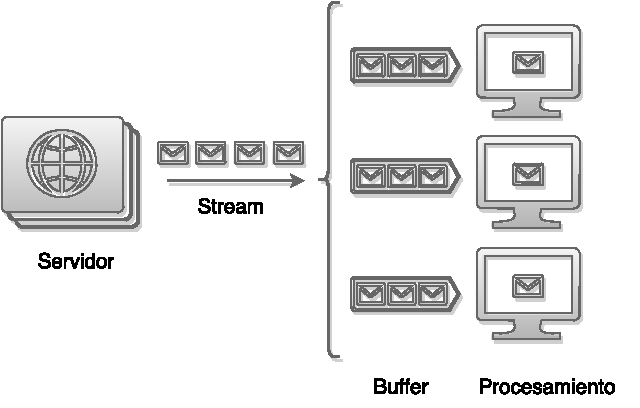
\includegraphics[scale=0.7]{images/Streaming.pdf}
  \caption{Flujo de datos entre el servidor y los clientes.}
  \label{fig:streaming}
\end{figure}

Este tipo de técnica es útil cuando se desea procesar información en tiempo real, siendo relevante la temporalidad de los datos, como la reproducción \textit{online} de material multimedia. Los datos emanados por el \textit{streaming} pueden ser utilizados para el análisis y procesamiento de un SPS (Sistema de Procesamiento de \textit{Stream}). Un ejemplo de esto, es la \textit{Streaming API} proporcionada por Twitter, donde esta información se puede utilizar para estudiar los \textit{tweets}, los \textit{trending topic} o los \textit{hashtag} más utilizados para casos específicos, como campañas electorales o desastres naturales.

\section{Stream processing}
\label{sec:streamProcessing}

\textit{Stream processing} es un paradigma de programación, el cual está orientado al procesamiento de un flujo de datos en tiempo real. Se centra en la programación de aplicaciones que puedan procesar la información en el momento, utilizando los recursos del sistema de forma paralela o distribuida para cumplir su objetivo, de tal manera que su procesamiento sea lo más cercano al tiempo real \citep{ChakravarthyJ09}.

Dentro de las aplicaciones existentes en el procesamiento de \textit{stream}, están el monitoreo de signos vitales, detección de fraudes, reproducción de videos \textit{online}. Para el funcionamiento correcto de estas aplicaciones, es necesario cumplir con ciertas características. Es por esto que se han propuesto ciertos requerimientos para el procesamiento continuo de datos \citep{andrade2014fundamentals}, los cuales son desglosados a continuación:

\begin{itemize}
	\item \textbf{Procesamiento de grandes cantidades de datos}: esto significa que al tratar de procesar los datos, no se puede guardar en una base de datos y luego procesarlos, como en general lo realizan los sistemas de \textit{bash processing}. Por lo tanto es necesario otro mecanismo que pueda procesarlos mientras va llegando la información entrante. Por lo que al utilizar \textit{stream processing} soluciona este problema, dado que la información entrante es procesada a medida que van llegando los datos.
	\item \textbf{Limitaciones de ancho de banda y latencia}: se refiere a la comunicación que existe por parte del proveedor de datos, de tal manera que no sea una limitante en el procesamiento de los datos el ancho de banda o la latencia existente. Esto es importante, dado que no sirve un sistema de estimación de la bolsa del mercado con una latencia considerable, de tal manera que envíe datos obsoletos. Siempre se debe mantener una baja latencia, para poseer los datos lo más cercano al tiempo real.
	\item \textbf{Procesamiento de datos heterogéneos}: en su mayoría, los datos poseen distintos formatos, contenidos y niveles de ruido, por lo que es necesario realizar una normalización de estos, de tal manera de estandarizar el procesamiento.
	\item \textbf{Proporcionar alta disponibilidad a largo plazo}: es importante poseer un constante flujo de información, que sea estable y persistente en el tiempo, de tal manera que esté procesando constantemente los datos para el propósito designado. Si analizamos el funcionamiento de los sistemas, estos poseen un porcentaje de fallas, y los SPS no son la excepción, por ello es importante contar con un mecanismo de tolerancia a fallos que permita reducir la pérdida de información. De no existir, se puede perder información, comprometiendo la precisión de los resultados y requiriendo de un mayor tiempo para recolectar la información perdida o alcanzar un estado similar.
\end{itemize}

\section{Sistemas de procesamiento de stream}
\label{sec:SPS}

Entre los diferentes motores de procesamiento de datos masivos, existen los sistemas de procesamiento de \textsl{stream}, los cuales reciben grandes cantidades de datos que deben procesar de forma distribuida y en tiempo real, de ahora en adelante hablaremos de procesamiento \textsl{online} para hacer referencia al tiempo real. Para realizar esto, se requiere un cambio en el paradigma tradicional de \textsl{bash processing}, el cual almacena los datos, los que posteriormente son procesados de forma \textsl{offline} \citep{HawwashN14}. Este cambio implica el análisis sin almacenar los datos, por lo que estos fluyen mientras son procesados.

El paradigma utilizado se basa en grafos de procesamiento como muestra la Figura \ref{fig:grafo}, donde los operadores corresponden a las vértices del grafo, como por ejemplo analizadores de sentimientos, filtros de palabras o algún algoritmo en particular, y las aristas corresponden a los flujos de datos entre un operador y otro \citep{Shahrivari14}. Además de esto, los datos proporcionados son originados por un ente externo, ya sea \textit{streaming} de redes sociales, estadísticas del monitoreo de un sistema, o transacciones en la bolsa de comercio, la cual entrega los datos iniciales a los primeros operadores del grafo \citep{AppelFFB12}.

\begin{figure}[ht!]
  \centering
    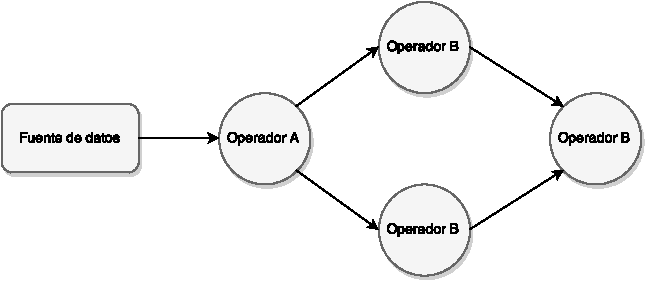
\includegraphics[scale=1]{images/SPS.pdf}
  \caption{Ejemplo de modelo de SPS.}
  \label{fig:grafo}
\end{figure}

Cabe destacar que los SPS son distribuidos, es decir, cada uno de los vértices del grafo son alojados en un nodo físico disponible en el ambiente en que se aloja el sistema, ya sea un \textit{cluster}, un \textit{grid} o un \textit{cloud}. Para lograr la comunicación entre los operadores, se utilizan sistemas anexos especialmente diseñados para este tipo de tareas, como Apache ZooKeeper \citep{HuntKJR10}. Este sistema es un servicio centralizado que mantiene la información de configuración y sincronización de las aplicaciones distribuidas que se posean. Por lo tanto, cada nodo al registrarse al servidor central, éste se encarga de señalar los nodos disponibles para la interacción entre ellos.

Las principales aplicaciones que se le dan a estos SPS, están orientadas al manejo de grandes cantidades de datos, las cuales deben ser procesadas para obtener información o estadísticas, como es el caso de detección de fraudes, recolección de información en caso de desastres o análisis de la interacción en las redes sociales. Para efectuar un procesamiento en tiempo real de los datos, \citep{StonebrakerCZ05} establece los siguientes requerimientos:

\begin{itemize}
	\item \textbf{Baja latencia}: este concepto está asociado con la comunicación fluida entre los distintos nodos del sistema, de tal manera que no existan altos \textit{delay} o retrasos en el procesamiento.
	\item \textbf{Consultas SQL}: poder realizar consultas a una base de datos, sin perder las propiedades del SPS, como el procesamiento distribuido. Para esto, se debe realizar un cambio en la forma de ejecutar las consultas, debido que no sólo es necesario realizar la consulta, sino también que se puedan unir las respuestas entregadas de forma paralela. Dado lo anterior, se hace necesario diseñar un sistema que cumpla con operadores adicionales a los utilizados en las consultas tradicionales por sistemas centralizados.
	%\item \textbf{Manejo de fallas en el flujo de dato}: es importante poseer sistemas que no se preocupen de la pérdida en los datos, debido que se posee como premisa que se van a perder datos en el procesamiento de estos, ya sea por las colas, \textit{delays} u otro problema asociado al procesamiento o la fuente de datos. Por lo tanto, al modelar la aplicación no es necesario lidiar con este tipo de fallas.
	\item \textbf{Generar resultados predecibles}: cuando se realizan consultas en el sistema, existe la posibilidad que sean correctas sólo por un período de tiempo, debido a alguna falla en el sistema que genere una pérdida en el estado del operador. Por lo tanto, es necesario garantizar que el resultado sea determinístico y persistente en el tiempo, ya sea respaldando la información u otro mecanismo, de tal manera que si se realiza una consulta, el resultado sea consistente u homólogo con el transcurso del tiempo.
	\item \textbf{Integrar almacenamiento y flujo de datos}: en general, cuando se trabaja con procesamiento de datos, es importante guardar estados en el sistema, de tal manera que los datos entrantes vayan verificando, modificando o eliminado la información que se posea. En un operador que cuente palabras, es necesario soportar variables que guarden las estadísticas de la información entrante. Otro tema importante es la uniformidad de los datos, como se había explicado anteriormente, en general se trabaja con datos heterogéneos, por lo que se requiere estandarizarlos para su procesamiento, de tal manera que no exista una discordancia en la información procesada.
	\item \textbf{Garantizar la seguridad y disponibilidad de los datos}: este requerimiento está orientado en poseer mecanismos de \textit{checkpoint}, técnica utilizada para respaldar el estado del operador cada cierto período de tiempo, y tolerancia a fallas. Por lo que en caso de existir alguna falla, el sistema pueda volver a estar disponible y sin perder una cantidad considerable de información, ya sea en las estadísticas o estados del sistema.
	\item \textbf{Partición y escalabilidad automática de las aplicaciones}: es importante también distribuir la carga entre los distintos procesadores o máquinas, deseando idealmente una escalabilidad incremental. Esto significa que el flujo de datos sea entregado a los distintos recursos que se poseen, y en caso de necesitar más recursos incrementarlos \citep{bookTanenbaum}. Si bien no sucede siempre, se espera que esto sea automático y transparente.
	\item \textbf{Procesamiento y respuesta instantánea}: cuando se plantea el uso de los SPS, se apuesta por un sistema que entregue respuestas en un tiempo lo más cercano al real. Este requerimiento hace necesario lidiar posibles sobrecargas de los operadores, las cuales afectan al rendimiento del sistema. Por lo tanto, se hace necesario abordar estos posibles escenarios proveyendo una solución de bajo \textit{overhead}, esto quiere decir con bajo costo de implementación o recursos necesarios para su funcionamiento, aumentando así la eficiencia y el rendimiento del sistema.
\end{itemize}

Cada sistema de procesamiento de \textsl{streaming} está basado en un modelo de procesamiento en particular. Por ejemplo, S4 utiliza el modelo de procesamiento \textsl{push} \citep{s4yahoo}, y Storm el modelo \textsl{pull} \citep{stormtwitter}.

El primer modelo llamado \textit{push}, consiste en el envío de datos desde el operador. La ventaja de este modelo empleado por S4 radica en la abstracción en el envío de datos, sin embargo no asegura el procesamiento de estos, debido a que no existe un mensaje de respuesta al ser entregado al operador. En la Figura \ref{fig:sps-push} se puede ver el Operador A como envía los datos al Operador B, donde en caso que el Operador B esté procesando un dato, éste lo guarda en cola. Debido a la forma en como se realiza el envío del evento, éste no asegura que llegue efectivamente, en caso que suceda una falla en la comunicación, habiendo una abstracción en el envío de los eventos por parte del operador emisor.

\begin{figure}[ht!]
  \centering
    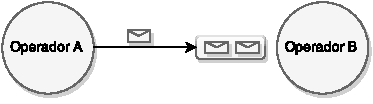
\includegraphics[scale=1]{images/SPS-Push.pdf}
  \caption{Modelo push de procesamiento.}
  \label{fig:sps-push}
\end{figure}

Por otra parte, el segundo modelo llamado \textit{pull}, se basa en la petición de datos a un operador, por lo que son enviados solo si son requeridos. Si bien este modelo asegura procesamiento de los datos, genera una menor abstracción al programador, dado que en el primer modelo sólo se indica a que operador deben ir los datos, en cambio en el segundo se debe indicar quién lo envía y quién lo recibe. En la Figura \ref{fig:sps-pull} (a) se observa que existen dos operadores, donde se solicita por parte del Operador B el envío de un dato para ser procesado, para que posteriormente en la Figura \ref{fig:sps-pull} (b) el Operador A envía el dato para que posteriormente sea procesado por el Operador B.

\begin{figure}[ht!]
  \centering
    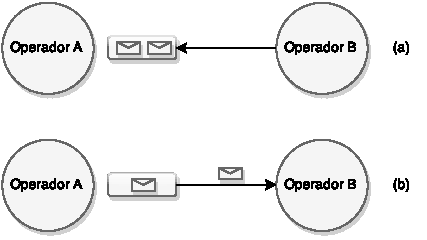
\includegraphics[scale=1]{images/SPS-Pull.pdf}
  \caption{Modelo pull de procesamiento.}
  \label{fig:sps-pull}
\end{figure}

\subsection{S4}
S4 (Simple Scalable Streaming System) \citep{s4yahoo} es un sistema de propósito general, distribuido y escalable que permite diseñar aplicaciones pueden procesar flujos de datos de forma continua y sin restricciones. S4 está inspirado en MapReduce \citep{2010Lin}, y está diseñado en el contexto de minería de datos y algoritmos de aprendizaje de máquina en Yahoo! Labs para sistemas de publicidad \textsl{online}. Cada evento en S4 es descrito como un par (clave, atributo), cuyos pares pueden ir agregándose a medida que sea necesario. La unidad básica son los elementos de procesamiento (PEs, por sus siglas en inglés). Los PEs pueden emitir o pueden publicar resultados y son alojados en servidores llamados nodos de procesamiento, llamados PNs. Los PNs son responsables de escuchar eventos, rutear eventos a los PEs del nodo y despachar eventos a través de la capa de comunicación. Los eventos son encaminados usando una función de \textsl{hashing} sobre los valores de los atributos hacia el PE apropiado. Para este fin, en la capa de comunicación utiliza Apache ZooKeeper \citep{HuntKJR10}, el cual provee manejo de \textit{clusters} y reemplazo automático de nodos que fallan. S4 usa encaminamiento estático, es parcialmente tolerante a fallas, y no posee mecanismos de balanceo dinámico de carga.

\subsection{Storm}
Storm \citep{bookstorm} es una plataforma similar a S4, orientada a la computación de flujos de datos en tiempo real de forma escalable. El modelo de programación está basado en dos primitivas básicas para la transformación de flujos de datos que deben ser implementados de acuerdo a la lógica de las aplicaciones: \textit{Spouts} y \textit{Bolts}. Un \textit{Spout} es una fuente de flujo de datos y un \textit{Bolt} hace una transformación de un solo paso sobre el flujo de datos, creando un nuevo flujo basado en la entrada que recibe. Transformaciones complejas requieren múltiples \textit{Bolts}, los cuales crean topologías o grafos, el nivel más alto de abstracción en Storm. La plataforma soporta tolerancia a fallas a través de un proceso maestro llamado Nimbus \citep{MiaoYJ14}, el cual garantiza el procesamiento de todos los mensajes a través del uso de una base de datos para su almacenamiento. Sin embargo, esta base de datos es su mayor desventaja respecto de S4 puesto que no es completamente distribuida. Storm define diferentes técnicas para el particionamiento de \textit{streams} de datos y para la paralelización de \textit{Bolts}, por lo tanto la asignación de máquinas para alguna actividad debe efectuarse de forma manual, lo que complica el desarrollo de aplicaciones. Al igual que S4, Storm usa Apache ZooKeeper \citep{HuntKJR10} en la capa de comunicación.

\section{Elasticidad}
\label{sec:elasticidad}

La propiedad de elasticidad en el área de \textit{Cloud Computing} o \textit{SPS}, está relacionado con la capacidad que el sistema tiene de adaptarse dinámicamente a las condiciones variables del sistema, como por ejemplo el tráfico. Esto quiere decir que aumente o disminuya los recursos que se utilicen, para que funcione de manera eficiente.

En el caso de \textit{Cloud Computing} existen estudios que han trabajado con esta propiedad como \citep{GongGW10, NguyenSGSW13, LehrigEB15}, donde el sistema se comporta de forma elástica, determinando dinámicamente la cantidad de máquinas virtuales necesarias en el sistema. Por otra parte, en los SPS, existen trabajos como \citep{GedikSHW14, IshiiS11, SchneiderAGBW09, MadsenTZ14, GulisanoJPSV12}, en que el sistema de forma dinámica determina la cantidad de operadores necesarios para realizar una tarea en específico, como se ve representando en la Figura \ref{fig:elasticidad}, donde la cantidad de operadores B cambia dinámicamente según el rendimiento del sistema.

\begin{figure}[!ht]
	\centering
	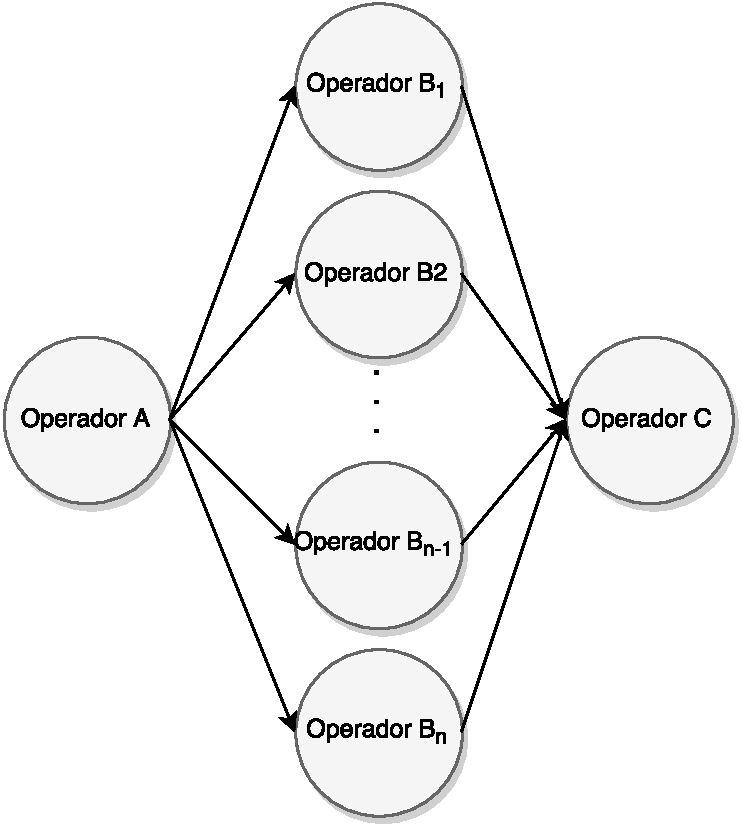
\includegraphics[scale=0.55]{images/Elasticidad.pdf}
	\caption{Elasticidad en un SPS.}
	\label{fig:elasticidad}
\end{figure}

Un ejemplo práctico de elasticidad es el supermercado, donde se debe considerar la cantidad de cajas necesarias para atender de manera eficiente los $n$ clientes que van llegando en un período de tiempo. Si se estudia el período de la mañana, en general, se tiene un bajo flujo de personas que acude al supermercado, en comparación con la tarde, pero alto comparado la medianoche. Por lo tanto, en los horarios de la tarde es necesario poseer una mayor cantidad de cajas disponibles que en la mañana, disminuyendo la cantidad nuevamente cuando el horario bordea la medianoche, adaptándose de forma elástica la cantidad de cajas disponibles en el supermercado.

En el trabajo realizado, se propone un sistema elástico dada la demanda de los distintos operadores. De esta manera, según el tráfico existente aumentan o disminuyen los operadores, de tal manera que trabaje de manera dinámica y de forma óptima.

\section{Procesos estocásticos}
\label{sec:procesosEstocasticos}

Se define proceso estocástico como una colección de variables aleatorias {$X_t$, con $t ~ \epsilon ~ T$}, las cuales están determinadas por algún comportamiento en el tiempo $t$. Esto significa que cada variable está tratada de forma discreta en el tiempo, sin poseer un proceso determinístico entre sus variables, es decir, que las variables dependan de la historia \citep{taylor2014introduction}.

Por lo tanto, se puede definir un estado como el posible comportamiento que puede tener una variable aleatoria en el sistema. Un ejemplo de esto es un modelo que contemple tres estados: estable, inestable y ocioso, y según el valor de la variable aleatoria, vaya cambiando de un estado a otro. Un caso de estudio utilizando el concepto de estados son las cadenas de Markov, las cuales consideran distintos estados, donde cada uno representa un comportamiento del sistema \citep{de1978calculus}.

Como se mencionó anteriormente, las cadenas de Markov son procesos estocásticos, las cuales se utilizan para soportar la predicción de carga en el modelo propuesto \citep{GongGW10}. De esta manera, se definen estados que son independientes en el transcurso del tiempo. Esto fue pensando con el fin de realizar análisis a futuro, tomando en consideración los datos \textit{a priori}.

\subsection{Cadena de Markov}
\label{subsec:cadenaMarkov}

Sea $X_t$ el valor de una variable aleatoria $X$ en un tiempo $t$, donde el conjunto de todos los valores posibles para $X$ se llama espacio de estado \citep{ching2006markov}. La variable aleatoria es un proceso de Markov si las probabilidades de transición entre dos estados cualquiera de $\Omega$ (definido como el universo de posibles estados), sólo depende del estado actual, como se denota en la Ecuación \ref{eq:defMarkov} y gráficamente en la Figura \ref{fig:procesoMarkov}. Cabe destacar que este tipo de proceso es un caso específico de los procesos estocásticos.

\begin{equation} \label{eq:defMarkov} 
	P_r(X_{t+r} = S_j | X_0 = S_k ; X_1 = S_l ; ... ; X_t = S_i) = P_r(X_{t+1} = S_j | X_t = S_i)
\end{equation}

\begin{figure}[ht!]
  \centering
    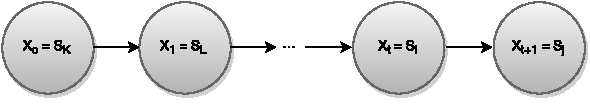
\includegraphics[scale=0.6]{images/ProcesoMarkov.pdf}
  \caption{Proceso de Markov.}
  \label{fig:procesoMarkov}
\end{figure}

Una cadena de Markov es una secuencia de variables aleatorias generadas por un proceso de Markov, como se denota en la Ecuación \ref{eq:cadenaMarkov}.

\begin{equation} \label{eq:cadenaMarkov}
	(X_0, X_1, X_2, ..., X_{n-1}, X_{n})
\end{equation}

La Ecuación \ref{eq:transicionMarkov} se define por sus probabilidades de transición. En la Figura \ref{fig:cadenaMarkov} se muestra un ejemplo de la transición del estado $i$ al estado $j$, dada la probabilidad $P_{ij}$.

\begin{equation} \label{eq:transicionMarkov}
	P_{ij} = P_r(i \rightarrow j) = P_r(X_{t+1} = S_j | X_t = S_i)
\end{equation}

\begin{figure}[ht!]
  \centering
    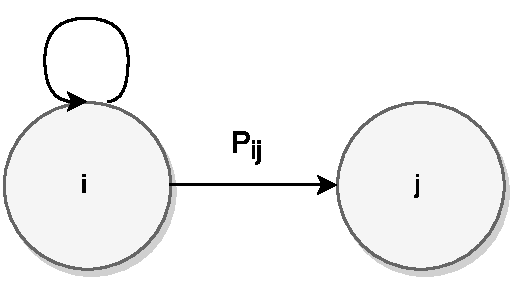
\includegraphics[scale=0.6]{images/CadenaMarkov.pdf}
  \caption{Cadena de Markov.}
  \label{fig:cadenaMarkov}
\end{figure}

En la Ecuación \ref{eq:matrizTransicion} se presenta una matriz de transición de finitos estados, donde la probabilidad de pasar de un estado a otro está determinado por una posición de la matriz, tomando en consideración que la suma de todas las transiciones de un estado debe ser igual a 1.

\begin{equation} \label{eq:matrizTransicion}
	P =
	\begin{bmatrix}
		P_{1,1} & P_{1,2} & \cdots & P_{1,n} \\
		P_{2,1} & P_{2,2} & \cdots & P_{2,n} \\
		\vdots  & \vdots  & \ddots & \vdots  \\
		P_{n,1} & P_{n,2} & \cdots & P_{n,n} \\
	\end{bmatrix}
	\hspace*{1cm} \sum_{j=1}^{n} P_{ij} = 1 ; \forall i
\end{equation}

En la Figura \ref{fig:ejCadenaMarkov} se muestra un ejemplo de una cadena de Markov simple, donde se analiza la probabilidad del clima de mañana dado el clima de hoy día. Como se puede observar, no se considera la historia del clima en la semana, sólo el del caso actual, lo cual es definido en los procesos estocásticos. Dada las probabilidades que transite de un clima a otro, se puede ver en la Ecuación \ref{eq:ejCadenaMarkov} la matriz de transición resultante.

\begin{figure}[ht!]
	\centering
	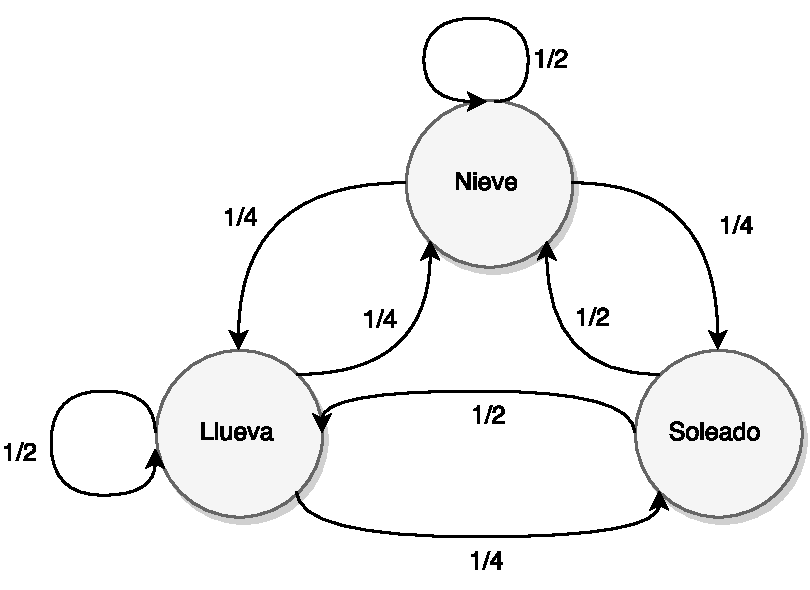
\includegraphics[scale=0.5]{images/EjCadenaMarkov.pdf}
	\caption{Ejemplo de cadena de Markov.}
	\label{fig:ejCadenaMarkov}
\end{figure}

\begin{equation} \label{eq:ejCadenaMarkov}
	P =
	\begin{bmatrix}
		\frac{1}{2} & \frac{1}{4} & \frac{1}{4} \\
		\frac{1}{2} & 0 & \frac{1}{2} \\
		\frac{1}{4} & \frac{1}{4} & \frac{1}{2}
	\end{bmatrix}	
\end{equation}

Si se desea saber la probabilidad que la cadena esté en el estado $S_i$ en el tiempo $t+1$, está dada por la ecuación de Chapman-Kolmogórov \citep{Papoulis1984}:

\begin{equation} \label{eq:chapman-kolmogorov1}
\begin{split}
	\Pi_{i} (t+1) &= P_r(X_{t+i}=S_i) \\
				  &= \sum _{k} P_r(X_{t+i} = S_i / X_t = S_k)·P_r(X_t = S_k)\\
				  &= \sum _{k} P_r(X_{t+i} = S_i / X_t = S_k)·\Pi_{k} (t)
\end{split}	
\end{equation}

En notación matricial:

\begin{equation} \label{eq:chapman-kolgorov2}
\begin{split}
	\Pi_{(t+1)} &= \Pi_{(t)}P\\
	\begin{bmatrix}
		\Pi_1 & \Pi_2 & \Pi_3
	\end{bmatrix} _{(t+1)}
	&= \begin{bmatrix}
		\Pi_1 & \Pi_2 & \Pi_3
	\end{bmatrix} _{(t)}
	\begin{bmatrix}
		P_{1,1} & P_{1,2} & \cdots & P_{1,n} \\
		P_{2,1} & P_{2,2} & \cdots & P_{2,n} \\
		\vdots  & \vdots  & \ddots & \vdots  \\
		P_{n,1} & P_{n,2} & \cdots & P_{n,n}
	\end{bmatrix}
\end{split}
\end{equation}

Usando recurrencia, se puede calcular la distribución estacionaria como se muestra la Ecuación \ref{eq:chapman-kolgorov3}, la cual indica el comportamiento a futuro de la cadena de Markov, dado los estados y transiciones que éste posee.

\begin{equation} \label{eq:chapman-kolgorov3}
\begin{split}
	\Pi (t) &= \Pi (t-1)P \\
				  &= \Pi (t-2)P^{2}\\
				  &= \Pi (0)P^{t} ; \Pi (0): \text{distribución inicial}
\end{split}
\end{equation}

\subsection{Trabajo relacionado}
\label{subSec:markovTrabajo}
Existen modelos predictivos que están basados en modelos matemáticos, los cuales simulan el comportamiento del sistema, ya sea del flujo o de la carga de un operador, de tal manera que pueden predecir cual es su estado en un tiempo futuro. En general, para poder realizar una predicción se analizan las variables en una ventana de tiempo, para posteriormente aplicar un modelo matemático que prediga la variación del sistema en la próxima ventana de tiempo que se tiene estipulada.

Dentro de las aplicaciones que se han realizado con modelos predictivos, se encuentra PRESS \citep{GongGW10}. En este sistema orientado a \textit{Cloud Computing} \citep{bookDistrSys}, analiza la cantidad de recursos disponibles, ya sea la memoria disponible o el uso promedio de CPU en las máquinas virtuales que se disponen en el \textit{Cloud}. Para realizar la predicción del estado del sistema, se aplica un modelo basado en cadenas de Markov, tomando sus estados como ventanas de tiempo en un determinado período. De esta manera, se analiza el estado del sistema en un tiempo en específico, para analizar si posee correlación con algún estado de la cadena de Markov, para posteriormente ver la transición de ese estado a otro y construir la matriz de transición. Posteriormente, con la ecuación de Chapman-Kolmogorov, se calcula la distribución estacionaria de la matriz de transición, de tal manera de saber en que estado está en la próxima ventana de tiempo, para finalmente analizar si es necesario algún cambio en el sistema.

Dentro de la misma línea de modelos predictivos, existe el sistema AGILE \citep{NguyenSGSW13} para \textit{Cloud Computing} que modifica las máquinas virtuales de forma elástica en un \textit{Cloud}. Lo que se realiza en este trabajo es aplicar la transformada de Fourier \citep{falk2012first} a series temporales, obtenidas mediante el muestreo de la carga de CPU en una ventana de tiempo. Luego, la función resultante se analiza con distintas frecuencias, de tal manera de solicitar la predicción de la próxima ventana de tiempo a cada una de las funciones creadas. De esta manera, se sintetizan todas predicciones realizadas por cada función para analizar el comportamiento del sistema en la próxima ventana de tiempo, y ver si es necesario aumentar o disminuir recursos de éste.

\section{Teoría de colas}
\label{sec:teoriaColas}

La teoría de colas se centra en el estudio matemático de las colas existentes en un sistema, cuyo caso de estudio es el desbordamiento de peticiones por parte del cliente al servidor \citep{queueingtheory}. En la Figura \ref{fig:teoriaColas} se muestra un ejemplo de un sistema basado en teoría de colas, donde existe $n$ productores que envían cierto flujo de datos a los $m$ servidores disponibles, y en caso de no estar disponibles, se genera una cola de espera en el sistema.

\begin{itemize}
	\item \textbf{Productor}: es quién provee la fuente de entrada para el servidor, de tal manera que procese según la necesidad que se posea.
	\item \textbf{Cola o línea de espera}: la cual está encargada de almacenar la información emanada por el productor en caso que los servidores estén ocupados, para que posteriormente sean procesados.
	\item \textbf{Servidor}: es quién procesa la información disponible en la cola, de tal manera de entregar una fuente de salida con los datos o información deseada.
\end{itemize}

\begin{figure}[!ht]
	\centering
	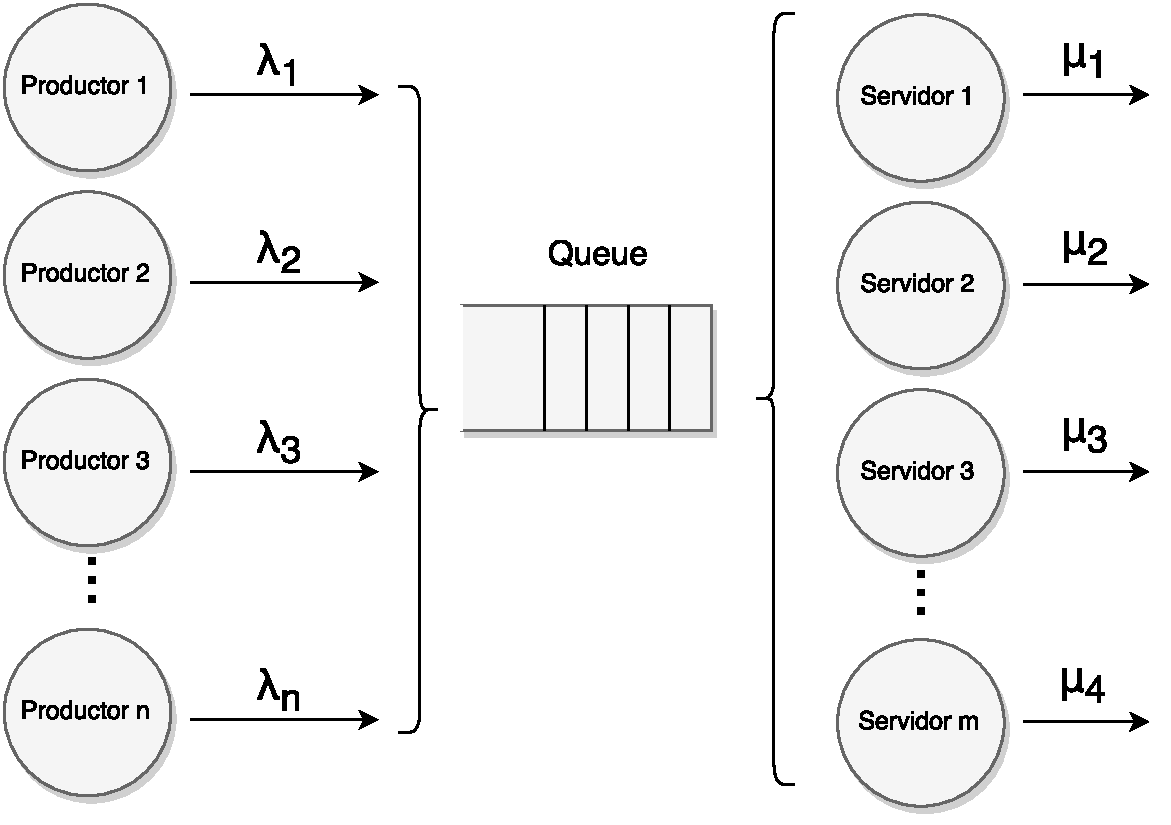
\includegraphics[scale=0.6]{images/TeoriaColas.pdf}
	\caption{Ejemplo de un sistema basado en teoría de colas.}
	\label{fig:teoriaColas}
\end{figure}

Además de esto, se tienen ciertos componentes importantes en el sistemas, definidos a continuación:
\begin{itemize}
	\item \textbf{Tasa de llegada}: denotado $\lambda$, es la cantidad de datos, eventos o información que van llegando en un determinado período de tiempo, la cual está determinada por los productores que existan en el sistema.
	\item \textbf{Tasa de procesamiento}: denotado $\mu$, también llamado tasa de servicio, es la cantidad de datos, eventos o información que salen del sistema, producto del procesamiento provisto por cada servidor.
	\item \textbf{Tasa de rendimiento}: denotado $\rho$, es el porcentaje de utilización del sistema, donde $\rho = \frac{\lambda}{s\mu}$, siendo $s$ la cantidad de servicios disponibles, definiendo así un sistema estable si es que $\rho < 1$, dado que la capacidad de procesamiento es mayor que la tasa de llegada.
	\item \textbf{Disciplina de la cola}: significa el método utilizado para extraer los datos encolados en el sistema, para esto puede aplicarse los métodos \textit{FIFO}, \textit{LIFO}, \textit{RSS}, entre otros.
\end{itemize}

Este tipo de modelos se puede aplicar a los SPS, debido que el operador emisor o la fuente de datos es el productor, y el operador receptor es el servidor del sistema. Por lo que existe un problema interesante a analizar debido a las posibles sobrecargas en los operadores. Por ejemplo, si se tiene un operador con una tasa de llegada $\lambda$ y una tasa de servicio $\mu$, donde $\mu < \lambda$, se tiene un sistema inestable, debido que se procesa más lento de lo que llegan los datos. Esto genera colas por lo que es necesario un aumento del rendimiento del sistema, debido que $\rho > 1 $, lo que significa que el sistema se encuentra inestable, generándose colas en éste. Es por esto, que para estabilizar el sistema, es necesario modificar la cantidad de réplicas existentes de ese operador del SPS, de tal manera de mejorar el rendimiento del sistema.
\chapter{Estado del Arte}
\label{cap:estadoDelArte}

\section{Sistemas de Procesamiento de \textit{Streaming}}

Entre los diferentes motores de procesamiento de datos masivos, existen los motores de \textsl{streaming}, los cuales reciben grandes cantidades de datos que deben procesar de forma distribuida y \textsl{online}. Para realizar esto, se requiere un cambio en el paradigma \textsl{bash processing}, el cual guarda los datos en una base de datos, los que posteriormente son procesados de forma \textsl{offline} \citep{HawwashN14}, a uno que procese de forma \textsl{online}. Por lo que el paradigma cambia a uno basado en grafos, donde a través del cual fluye un \textsl{stream} de datos que es procesamiento por el conjunto de operadores que lo componen, los operadores corresponden a las vértices del grafo, y las aristas a los flujos de datos preprocesados que salen del operador \citep{Shahrivari14}.

El modelo de procesamiento que se muestra en la Figura \ref{fig:grafo}, corresponde a un SPS (Sistema de Procesamiento de \textit{Streaming}). Los vértices corresponden a operadores, como por ejemplo analizadores de sentimientos, filtros de palabras o algún algoritmo en particular, y las aristas corresponden a los flujos de datos entre un operador y otro. Además de esto, se tiene una fuente de datos, la cual entrega los datos iniciales a los primeros operadores del grafo \citep{AppelFFB12}.

\begin{figure}[ht!]
  \centering
    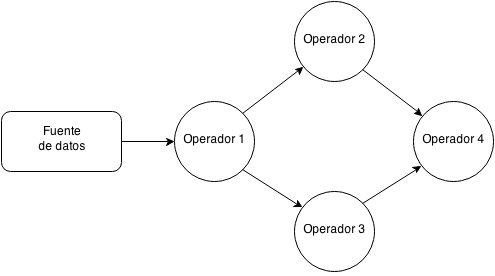
\includegraphics[scale=0.5]{images/Grafo.png}
  \caption{Ejemplo de modelo de SPE.}
  \label{fig:grafo}
\end{figure}

Cabe destacar que al ser distribuido los SPS, cada uno de las vértices del grafo serán alojadas en un nodo del ambiente que esté siendo almacenada, ya sea un \textit{cluster}, un \textit{grid} o un \textit{Infrastructure-as-Service}. Por lo que se debe realizar una comunicación entre los distintos nodos, para realizar el envío del flujo de un operador a otro.

Cada motor de procesamiento de \textsl{streaming} está basado en un modelo de procesamiento en particular. Por ejemplo, S4 está basado en el modelo de procesamiento \textsl{push} \citep{s4yahoo}, y Storm en el modelo \textsl{pull} \citep{stormtwitter}. El primer modelo consiste en el envío de datos desde el operador. La ventaja de este modelo empleado por S4 radica en la abstracción en el envío de datos, sin embargo no asegura el procesamiento de estos, debido a que no existe un mensaje de respuesta al ser entregado al operador. En cambio, en el segundo modelo se basa en la petición de datos a un operador, por lo que son enviados solo si son requeridos. Si bien este modelo asegura procesamiento de los datos, genera una menor abstracción al programador, dado que en el primer modelo sólo se programa a que operador debe ir, en cambio en el segundo se debe indicar quién lo envía y quién lo recibe.

Pues bien, independiente del método que se utilice, existe un problema en la distribución, dado el dinamismo de los datos a procesar, pudiendo generarse sobrecargas en algún operador. Esto se produce dado que la tasa de procesamiento es menor a la tasa de llegada, generando colas en el sistema \citep{queueingtheory}. Por ejemplo, si se posee una tasa de llegada $\lambda$ y una tasa de servicio $\mu$, donde $\mu < \lambda$, se generan colas en el sistema, debido que se procesa más lento de lo que llegan los datos. Como existen colas, es necesario un aumento del rendimiento del sistema, debido que $\rho > 1 $, donde se define $\rho = \frac{\lambda}{s\mu}$, siendo $s$ la cantidad de servicios disponibles.

\section{Balance de carga}

Dentro de la literatura se han encontrado distintas perspectivas al problema de balance de carga en un SPS (Sistema de Procesamiento de \textsl{Streaming}), las cuales consideran los recursos físicos o lógicos como problemas de la sobrecarga del sistema.

\subsection{Recursos físicos}
En esta perspectiva se toma en consideración la sobrecarga del sistema dado las limitantes físicas que éste posea, ya sea por condiciones de los recursos disponibles o por el ambiente de desarrollo. Para esto, se consideran distintos parámetros como umbrales, los cuales si son sobrepasados debe aplicarse alguna estrategia para aliviar la carga del sistema. Estos umbrales pueden ser el nivel SLO, porcentaje de CPU utilizada o disponibilidad de la memoria \citep{Dong06schedulingalgorithms}.

Una de las soluciones con la perspectiva anterior es el Borealis \citep{XingZH05}, donde considera la cantidad de carga de los nodos en ventanas de tiempo determinadas, las cuales serán manejadas por un coordinador centralizado. Por lo que este coordinador estará encargada de analizar los recursos del sistema, y en caso de sobrepase el umbral propuesto, se deberán emigrar los operadores que estén en ese nodo, para luego ser enviados a otro nodo candidato con menor cantidad de carga. Para elegir al nodo candidato, se realizó una análisis de la cantidad de correlación que existe entre el operador y el nodo candidato, de esta manera, no necesariamente iba a ser enviado a otro nodo con menor sobrecarga, sino también a uno que posea menor cantidad de mensajes. Dentro de los problemas que pueden existir en el sistema es la conexión entre los distintos nodos, por lo que para las pruebas se consideró un buen ancho de banda, de tal manera que aparente una red sin limitaciones de recursos.

Otra de las soluciones que se han propuesto es lo realizado por Flood \citep{Alves2010flood}, el cual es un DPS (\textit{Distributed data stream processing}) que considera ciertos factores físicos para agregar o eliminar máquinas virtuales que se provee del \textit{Infrastructure-as-Service}, como Amazon EC2. Para esto, se posee un administrador que considera las estadísticas en tiempo de ejecución como la cantidad de CPU utilizada, latencia o memoria disponible, las cuales considera para ver en que rango está de los umbrales establecidos, y posteriormente agregar o eliminar recursos de manera elástica.

\subsection{Recursos lógicos}
%A diferencia de la física, aquí se consideran los componentes lógicos del sistema, como por ejemplo, una sobrecarga en algún operador. De esta manera, en las distintas soluciones se pueden encontrar soluciones en cuanto a la carga existente en el operador o la cantidad de cola que posea, de tal manera, que estos sean los umbrales a considerar para generar una mejora en el sistema.

A diferencia de la física, en esta perspectiva se consideran los componentes lógicos del sistema, como la carga de un operador. Por lo que las distintas soluciones que se presentan, analizan la componentes como el flujo de datos o el tamaño de la cola de un operador, tomando esos parámetros como umbrales en los algoritmos implementados para realizar mejoras en el sistema.

% Enfoques de la perspectiva lógica

Dado esta perspectiva, se han presentando dos tipos de enfoques: el estático y el dinámico \citep{Gupta99loadsharing}. El primer enfoque está centrado en un modelo definido y fijo antes de la inicialización del sistema, sin considerar el estado del sistema. En cambio, el segundo enfoque está basado en un modelo que analizará el sistema según su estado en el transcurso de su ejecución.

%El primer enfoque se centra en la confección de un modelo definido y fijo antes de iniciar el sistema y que no varía en el tiempo. En cambio, el segundo se basa en la adaptación del sistema según su estado en tiempo de ejecución.

\subsection{Enfoque estático}

Este enfoque se ha implementando en distintos motores de \textsl{streaming}, donde no se depende del estado del sistema \citep{stormtwitter, s4}. De esta manera, no existe una interrupción en la ejecución o un cambio debido al estado del sistema \citep{CasavantK88}. Por lo tanto, no se considera variables como la carga o cola del operador, sólo se aplican técnicas que administren el flujo de los datos en el sistema.

%\textsl{Storm} utiliza la técnica de distribución de operadores según alguna política, tomando el enfoque estático \citep{stormtwitter}. El sistema configura el número de operadores que son necesarios para realizar una tarea, para que después estos sean repartidos en los distintos nodos disponibles según la política de \textit{Shuffle grouping}. Esta técnica basada en algoritmos de planificación \citep{bookScheduling}, consiste en distribuir los operadores en los distintos nodos utilizando una planificación \textsl{Round-Robin}, de tal manera que la cantidad de operadores sea uniforme en los nodos del sistema \citep{bookstorm}.

\textsl{Storm} utiliza distintas técnicas de distribución de las tuplas en los operadores según la política que se desee, todas tomando el enfoque estático \citep{stormtwitter}. Dentro de las políticas que existen son \textit{Shuffle grouping}, \textit{Fields grouping}, \textit{Partial Key grouping}, \textit{All grouping}, \textit{Global grouping}, \textit{None grouping}, \textit{Direct grouping} y \textit{Local grouping}.

La política de \textit{Shuffle grouping} se enfoca en distribuir las tuplas de forma homogéneas en los $n$ operadores que se encuentren en el grafo, utilizando la planificación \textit{Round-Robin} \citep{bookScheduling}, de esta manera la cantidad de tuplas se distribuye de forma homogénea en el sistema. Una de las principales fallas es que la tasa de procesamiento de las tuplas no siempre es la misma, por lo tanto puede existir una sobrecarga en un operador que le llegue mayor cantidad de tuplas con un mayor tiempo de procesamiento. Otra de las políticas muy utilizadas es \textit{Fields grouping}, la cual determina ciertas llaves a un operador determinado, es decir, si la llave fueran palabras desde una letra hasta otra letra serán procesadas por cierto operado. Si bien genera un determinismo en el procesamiento de las llaves, puede existir una sobrecarga de un operador, debido que una llave se repite con mayor frecuencia que otras \citep{bookstorm}.

%Otra técnica es el uso de la función \textsl{hash} \citep{RogawayS04} para distribuir los operadores en el grafo, como lo planteado en S4 \citep{s4yahoo}. Esto consiste en aplicar lo anterior a algún atributo del evento, mapeando el evento al operador que corresponda de los $n$ operadores disponibles según el valor de la función. Cabe destacar que si no existe un operador mapeado con la imagen de la función, el sistema clona uno existente evaluando el nuevo con la imagen de la función como identificador. De esta manera, esta técnica provee dinamicidad respecto a la cantidad de operadores en el sistema.

Por otra parte, se encuentra el funcionamiento de S4, cuya política es similar a la de \textit{Fields grouping} de Storm, la diferencia es que un operador no le corresponde un conjunto de llaves, sino que posee una llave única. Esto quiere decir que cada llave se le asigna un operador, y en caso de no existir un operador para el valor de esa llave, se creará un nuevo operador para esa llave. Debido a la infinidad de combinaciones en la llave, S4 recomienda aplicar una función \textit{hash} \citep{RogawayS04}, de esta manera el valor de la función determina el operador que procesará el dato y disminuirá la cantidad de operadores que deben estar disponibles. Esta técnica provee dinamismo en la cantidad de operadores en el sistema, pero al igual que la \textit{Fields grouping} puede sobrecargar un operador, debido que una llave posee mayor frecuencia que las otras.

Una ventaja del enfoque estático es el bajo costo de la implementación de los métodos, lo cual es beneficioso para sistemas con bajos recursos. Por otra parte, una desventaja existente es la sobrecarga de un nodo u operador, debido que no asegura que la cantidad de flujo sea repartido de forma homogénea. Si bien, no es una solución óptima, es un buen complemento para un modelo con el enfoque dinámico.

\subsection{Enfoque dinámico}

%Este enfoque está basado en el estado del sistema, donde según las variables y estado de cada uno de sus atributos, genera una acción en el sistema \citep{CasavantK88}. Esto significa que si el sistema posee alguna anomalía, como una sobrecarga en un operador o latencia entre distintos nodos, se realiza un cambio en el sistema, con el fin de solucionar estos problemas. Para poder dar una solución al problema de sobrecarga, se pueden utilizar dos tipos de modelos: reactivo y predictivo.

Este enfoque está basado en el estado del sistema, siendo esto el parámetro para optimizar el rendimiento del sistema \citep{CasavantK88}. Esto significa que si el sistema le surge una anomalía, como una sobrecarga o latencia entre nodos, es necesario realizar un cambio en el sistema, con el fin de solucionar estos problemas. Por lo que para solucionar estos problemas, se consideran dos modelos: el reactivo y el predictivo.

\paragraph{Reactivo}

Este modelo está basado en la detección de sobrecargas en el sistema a través de un monitor \citep{GulisanoJPSV12}, el cual recibe periódicamente las variables de cada uno los operadores, y en caso que sobrepase un umbral, se aplica una técnica para aumentar el rendimiento bajo una métrica dada. El umbral puede estar basado en el tiempo de procesamiento, el tamaño de la cola u otra variable del operador \citep{BhuvanagiriGKS06}. Por ejemplo, para realizar una optimización en el rendimiento general del sistema, se considera la tasa de procesamiento de cada operador, por lo que en caso de existir congestión en un operador, se procede a realizar una paralelización del operador, de tal manera que exista un operador adicional que pueda recibir un flujo de datos y realizar la misma operación que el operador sobrecargado \citep{SchneiderAGBW09}.

% Arreglar
Si bien estas soluciones en su mayoría son eficientes y poseen buen rendimiento, una de los principales problemas es que no analiza el comportamiento a futuro, debido que sólo analiza la situación en el momento, resolviendo el problema en el momento. Otro problema son los falsos positivos, debido que puede ser que en un momento exista un \textit{pick} de tráfico, pero esto era sólo un caso particular de un tiempo determinado, por lo que no era necesaria la mejora en el sistema.

\paragraph{Predictivo}

%El modelo predictivo está basado en modelos matemáticos que puedan simular la actividad del operador y predecir la carga de éste en tiempo futuro. En general, los pasos a seguir son en primer lugar determinar la carga de un operador en cierto período de tiempo, y segundo lugar aplicar un modelo matemático que prediga la carga en el próximo intervalo de tiempo. Un ejemplo de esto, es la predicción de carga de cada operador se realiza mediante modelos de Markov \citep{GongGW10}, de tal manera que con la iteración . Si bien lo anterior no ha sido implementando en el contexto de \textsl{Stream}, si se ha realizado en \textit{Cloud Computing} según la sobrecarga de los computadores \citep{NguyenSGSW13}.

Los modelos predictivos están basados en modelos matemáticos, los cuales simulan el comportamiento del sistema, ya sea del flujo o de la carga de un operador, de tal manera que pueda predecir como será su estado en un tiempo futuro. En general, para poder realizar una predicción se analiza las variables deseadas en una ventana de tiempo, para posteriormente aplicar un modelo matemático que prediga la variación del sistema en la próxima ventana de tiempo que se tiene estipulada.

Dentro de las aplicaciones que se han realizado con modelos predictivos, se encuentra PRESS \citep{GongGW10}. En este sistema lo que se analiza es la cantidad de recursos disponibles, ya sea la memoria disponible o el uso promedio de CPU, en las máquinas virtuales que se dispone en el \textit{Infrastructure-as-a-Service}. Para realizar la predicción del estado del sistema, se aplicó cadenas de Markov, tomando sus estados como ventanas de tiempo en un determinado período. De esta manera, se analiza el estado del sistema en un tiempo en específico, para analizar si posee correlación con algún estado de la cadena de Markov, para posteriormente ver la transición de ese estado a otro y generar la matriz de transición. Posteriormente, con la ecuación de Chapman-Kolmogorov \citep{Papoulis1984}, se calcula la distribución estacionaria de la matriz estacionaria, de tal manera de saber en que estado estará en la próxima ventana de tiempo, para finalmente analizar si es necesario algún cambio en el sistema.

Dentro de la misma línea, existe el sistema AGILE que modifica las máquinas virtuales de forma elástica en un \textit{Infrastructure-as-a-Service} \citep{NguyenSGSW13}. Lo que se realizó en este trabajo fue aplicar la transformada de Fourier a la carga de CPU en una ventana de tiempo determinada, donde la función resultante se analizó con distintas frecuencias, de tal manera de solicitar la predicción de la próxima ventana de tiempo a cada una de las funciones creadas. De esta manera, se sintetizan todas predicciones realizadas por cada función, para analizar el comportamiento del sistema en la próxima ventana de tiempo, y ver si es necesario aumentar o disminuir recursos de éste.

%Par esto, se analizarán distintos estados como cantidad de ventanas de tiempo que se consideren en un período determinado, por lo que posteriormente se analizará si cierto tiempo posee una correlación o no con cierto estado, de esta manera se analiza el cambio que surge de un estado a otro hasta generar una 

\section{Técnicas de balance de carga}

Existen distintas técnicas de balance de carga que utilizan alguno de los dos modelos presentados anteriormente, los cuales están enfocadas en mejorar al rendimiento del sistema en caso de existir una sobrecarga. Dentro de las técnicas existentes se encuentrán la planificación determinista \citep{XuCTS14, DongTS07}, descarte de eventos \citep{SheuC09}, migración \citep{XingZH05}, paralelización \citep{GulisanoJPSV12, IshiiS11, GedikSHW14} y replicación \citep{FernandezMKP13}.

\subsection{Planificación determinista}
%La planificación determinista \citep{DongTS07} se centra en la planificación según los recursos y estados del sistema \textit{a priori} según alguna métrica \citep{XuCTS14}. Una métrica utilizada es la frecuencia de datos estimada en un nodo u operador \citep{Ganguly09}. Esta técnica se utiliza, por ejemplo, en \textit{StreamIt} \citep{ThiesKA02}. Una de las limitaciones es que si bien realiza una predicción determinista de la frecuencia, no necesariamente es correcta a futuro, por lo que no se puede predecir las tasas de tráfico en el transcurso del procesamiento, sino sólo estimarlas al comienzo de la ejecución del sistema.

La planificación determinista se centra en los conocimientos \textit{a priori} del sistema, esto significa que se consideran las variables del entorno que se poseen y respecto a esto se toma una decisión de como debe actuar el sistema. En otras áreas, como red de sensores, se utiliza esta técnica en el envío de estadísticas de dispositivos móviles, los cuales manejan información \textit{a priori} de donde están los sensores, de tal manera de determinar según la intensidad de la frecuencia, localización o clima, a dónde debe enviar la señal para que se recolecte la información correspondiente \citep{DongTS07}.

En el caso de \textit{Streaming}, se han realizado varias análisis respecto al análisis de la estimación de frecuencia de \textit{data stream} en el sistema. Para poder realizar esto, se han considerado modelos matemáticos, tomando ventanas de tiempo de la frecuencia predicha y la real, para posteriormente generar con los datos una función que represente la frecuencia estimada del operador \citep{Ganguly09}. Pero no sólo se han considerado modelos matemáticos, sino también algoritmos que determinan la frecuencia del sistema dado el flujo de datos que se posee \citep{BhuvanagiriGKS06}.

Una de las limitaciones es que si bien realiza una predicción determinista de la frecuencia, no necesariamente es correcta a futuro. Esto se debe a qué puede analizarse respecto al promedio, pero pueden surgir procesos anómalos en el transcurso de la ejecución que generará una sobrecarga en el sistema. Por lo tanto, la estimación al realizarse \textit{a priori}, sólo podrá considerar el inicio del sistema o ventanas de tiempo, por lo que puede existir un porcentaje de error considerable. Por otra parte, se considera que posee mejor rendimiento esta técnica si es que la frecuencia es estacionaria.

\subsection{Load Shedding}
%Otra estrategia está orientada a descartar eventos de un operador sobrecargado, de tal manera de no generar colas en el sistema. Esta estrategia que si bien no está implementada en el sistema por defecto de S4, puede habilitarse \citep{s4}. Otro ejemplo, es la trasmisión de vídeo \textit{streaming}, donde se descartan los datos que son de baja calidad, para procesar en su mayoría información de alta calidad \citep{SheuC09}. Esta solución está pensada para disminuir la carga, perdiendo la exactitud de la información debido a la pérdida de datos. Por lo tanto existe una menor fiabilidad en el sistema en caso de realizar operaciones de transacción \citep{bookDistrSys}.

En los SPS también se encuentra la técnica de \textit{load shedding} o descarte de eventos, que consiste en descartar eventos del sistema en caso de existir un comportamiento anómalo. Por ejemplo, en la transmisión de \textit{video streaming}, al enviar el flujo de información existe un administrador que estará analizando el contenido a procesar, por lo que en caos de llegar datos de baja calidad, serán descartados por éste. De esta manera, al existir menor cantidad de datos que procesar, el sistema posee un mejor rendimiento, además de tener una mejor calidad en la visualización de los videos, dado que en su mayoría se procesan datos de alta calidad \citep{SheuC09}. 

En el mundo de los SPS, varios poseen este tipo de estrategia, como por ejemplo S4 \citep{s4}, doonde se establece una cota superior de eventos en cola, y en caso que su cola sea igual al límite establecido, los eventos entrantes serán descartados. Otro sistema que aplica esta técnica es Aurora \citep{aurora}, el cual se basa en procesamiento de datos por ventanas de tiempo, por lo que en caso de existir una ventana de tiempo con una mayor cantidad de eventos de lo estipulado, se descartará el exceso de eventos.

Si bien esta técnica es simple y de bajo costo, siendo pensada para la disminución rápida de carga, existe una baja en la precisión y fiabilidad del procesamiento de los datos. Por ejemplo, en el caso de la transferencia de video no es trascendental, dado que son pocos los pixeles perdidos, pero en una recopilación y análisis de estadísticas, esto dará una menor precisión de los datos procesados por el sistema, dado que puede perderse información que indique comportamientos de los datos estudiados.

\subsection{Migración}
%También se encuentra la migración, en el cual según el estado del sistema se migran los operadores de un nodo a otro. En \citep{XingZH05} se implementa   esta técnica, y si bien genera una menor carga en distintos nodos, produce un alto costo en la transferencia de los datos. Al realizar la transferencia de los datos, existe una menor tolerancia a fallos, a raíz de lo cual, se propone el uso de un búffer en el sistema, aumentando sus costos \citep{PittauACA07}.

\subsection{Fisión}
Desde otra perspectiva, existen las técnicas de paralelización y replicación, las cuales se utilizan en caso de sobrepasar un umbral, el cual depende de la carga de un operador, nodo, entre otras variables. El primero consiste en paralelizar una tarea, la cual está determinada por un conjunto de operadores, en otro nodo físico \citep{IshiiS11}. En cambio, la replicación consiste en replicar un operador a nivel lógico del grafo \citep{MadsenTZ14}. Una de las características que existen en este tipo de soluciones es la elasticidad, que consiste en la capacidad de aumentar o disminuir la cantidad de operadores según la necesidad del sistema.

Una aplicación de la técnica de paralelización según el enfoque estático, es la paralelización de tareas de Storm \citep{stormtwitterdoc}, donde un conjunto de operadores realizan una tarea, indicado la cantidad de tareas que se desean ejecutar paralelamente en el sistema. Un ejemplo aplicado de esta técnica según el enfoque dińamico es StreamCloud \citep{GulisanoJPSV12}, que dada la cantidad de consultas que van llegando al sistema, se paralelizan las tareas existentes. Uno de los problemas que surge en estos casos son las operaciones con estado, como lo son los contadores o algoritmos de orden. La solución planteada es poseer un operador que realiza la tarea de \textit{merge}, que consiste en recibir las salidas de las tareas paralelas, agrupando los datos y proporcionando una salida según lo realizado por cada uno de las operaciones \citep{GedikSHW14}.

Por otra parte, se usa la técnica de replicación en una aplicación diseñada por Fernández \citep{FernandezMKP13}. Ésta está enfocada en la replicación de operadores, la cual se activa si se detecta un cuello botella en el procesamiento de los datos. Para la detección, existe un monitor que está recibiendo la carga de cada uno de los procesos, y si es sobrepasado el umbral, debe realizar una petición de replicación al operador sobrecargado.

% ----------------------------------------------------------
% ----------- TERCERA PARTE --------------------------------
% \backmatter %Elimina la numeración
% ### Bibliografía de este documento ###
\bibliographystyle{apa-good}
\bibliography{referencias}

% ----------------------------------------------------------
% ----------- CUARTA PARTE ---------------------------------
\appendix
\addappheadtotoc %agregar Apéndice al índice. Si no tiene apéndices COMENTAR o BORRAR
% \noappendicestocpagenum %quitar número de páginas a los apéndices
% ### ANEXOS ###
\chapter{Conformación de matriz de transición}
\label{apendice:matrizTransicion}

En el Algoritmo \ref{alg:matrizTransicion} se puede apreciar la conformación de la matriz de transición dado la historia de un operador determinado.

\begin{algorithm}[!hb]
	\setstretch{1}
	\caption{Algoritmo para la conformación de la matriz de transición.}
	\label{alg:matrizTransicion}
	\begin{algorithmic}[1]
	\REQUIRE $rho$ Historial de procesamiento de tamaño $n$ del operador $\phi$.
	\ENSURE $\Gamma$ Matriz de transición del operador $\phi$.
	\STATE $\Gamma \leftarrow Matriz[3x3]$ \COMMENT {Matriz de transición}
	\STATE $\tau \leftarrow Arreglo[3]$ \COMMENT {Contador para la normalizaci\'on de los datos}
	\FOR {$i=1$ a $n$}
		\IF {$\rho_i < 0.5$ \AND $\rho_{i+1} < 0.5$}
			\STATE $\Gamma_{1,1}++$
			\STATE $\tau{1}++$
		\ELSIF {$\rho_i < 0.5$ \AND $0.5 \leqslant \rho_{i+1} \leqslant 1$}
			\STATE $\Gamma_{1,2}++$
			\STATE $\tau{1}++$
		\ELSIF {$\rho_i < 0.5$ \AND $\rho_{i+1} > 1$}
			\STATE $\Gamma_{1,3}++$
			\STATE $\tau{1}++$
		\ELSIF {$0.5 \leqslant \rho_{i} \leqslant 1.5$ \AND $\rho_{i+1} < 0.5$}
			\STATE $\Gamma_{2,1}++$
			\STATE $\tau{2}++$
		\ELSIF {$0.5 \leqslant \rho_{i} \leqslant 1.5$ \AND $0.5 \leqslant \rho_{i+1} \leqslant 1.5$}
			\STATE $\Gamma_{2,2}++$
			\STATE $\tau{2}++$
		\ELSIF {$0.5 \leqslant \rho_{i} \leqslant 1.5$ \AND $\rho_{i+1} > 1.5$}
			\STATE $\Gamma_{2,3}++$
			\STATE $\tau{2}++$
		\ELSIF {$\rho_i > 1$ \AND $\rho_{i+1} < 0.5$}
			\STATE $\Gamma_{3,1}++$
			\STATE $\tau{3}++$
		\ELSIF {$\rho_i > 1$ \AND $0.5 \leqslant \rho_{i+1} \leqslant 1.5$}
			\STATE $\Gamma_{3,2}++$
			\STATE $\tau{3}++$
		\ELSE
			\STATE $\Gamma_{3,3}++$
			\STATE $\tau{3}++$
		\ENDIF	
	\ENDFOR

	\FOR {$i=1$ a $3$}
		\IF{$\tau_{i} \neq 0$}
			\FOR {$j=1$ a $3$}
				\STATE $\Gamma_{i,j} \leftarrow \nicefrac{\Gamma_{i,j}}{\tau_{i}}$
			\ENDFOR
		\ENDIF
	\ENDFOR
	
	\RETURN $\Gamma$ \COMMENT{Retorno de la Matriz de transici\'on normalizada, la cual define la cadena de Markov}
	\end{algorithmic}
\end{algorithm} % Manuales de Usuario
\end{document}
%\\end
